\documentclass[12pt]{article}
\usepackage{graphicx}
\usepackage[utf8]{inputenc}
\usepackage{float}
\usepackage{placeins}
\usepackage[colorlinks=true, allcolors=blue]{hyperref}
\usepackage{fancyhdr}
\usepackage{tikz}
\usetikzlibrary{positioning}
\pagestyle{fancy}
\usepackage[english]{babel}

\fancyhf{}
\fancyhead[L]{\textbf{Progress Report}}
\fancyfoot[C]{\hspace{4cm}\thepage}

\usepackage{amsmath,booktabs,array,caption,xcolor,colortbl,multirow,siunitx}

\definecolor{lightgray}{gray}{0.9}
\newcolumntype{C}{>{\centering\arraybackslash}p{0.8cm}}

\usepackage{amsmath}
\newtheorem{example}{Example}
\usepackage{hyperref}
\graphicspath{{Figures/}}
\addtolength{\textwidth}{1in}
\addtolength{\textheight}{1in}
\addtolength{\evensidemargin}{0.5in}
\addtolength{\oddsidemargin}{-0.5in}
\addtolength{\topmargin}{-0.5in}

\usepackage{listings}
\lstset{
  basicstyle=\ttfamily\small,
  breaklines=true,
  frame=single,
  backgroundcolor=\color{lightgray},
  captionpos=b,
  numbers=left,
  numberstyle=\tiny\color{gray},
  keywordstyle=\color{blue},
  commentstyle=\color{green!60!black},
  stringstyle=\color{orange},
  language=Python
}

\title{\textbf{Network Intrusion Detection Using CNN-BiLSTM with Logit-Adjusted Focal Loss on the CSE-CIC-IDS2018 Dataset}\\[0.5em]
\large Progress Report — AI Detection Component}
\author{Walid Ichchou \\[0.3em]
\small Groupe 3 — IDS-Blockchain Project \\[0.3em]
Supervisor: Badr Hirchoua}
\date{\today}

\usepackage{mathpazo}
\renewcommand\familydefault{\rmdefault}

\usepackage{amsthm}
\theoremstyle{plain}
\newtheorem{lemma}{Fact}[section]
\newtheorem{conjecture}{Conjecture}[section]
\newtheorem{lema}{Lema}[section]

\newcommand{\jp}[1]{\textcolor{teal}{#1}}
\newcommand{\pe}[1]{{\color{red}{#1}}}
\sloppy

\begin{document}

\maketitle

\begin{abstract}
This report presents the data preprocessing pipeline and neural network training methodology developed for the intrusion detection component of the IDS-Blockchain project. The system operates on the CSE-CIC-IDS2018 benchmark dataset, classifying network flows into 15 traffic categories spanning benign traffic and 14 distinct attack families. We detail a streaming preprocessing pipeline capable of handling the full 16~GB dataset within a single-node RAM budget, and describe the design and training of a CNN-BiLSTM classifier augmented with multi-head attention pooling and logit-adjusted focal loss. The production model achieves a macro-averaged F1 score of \textbf{0.7711} on the held-out test set, surpassing the 2-layer BiLSTM baseline (0.7366) by 3.45 absolute points. Critical design decisions—per-flow classification without sliding windows, the pseudo-sequence reshape strategy, and the validated single-rebalancing-lever constraint—are discussed with both technical justification and empirical evidence.
\end{abstract}

\tableofcontents
\clearpage

\listoffigures
\newpage
\listoftables
\newpage

\section*{Introduction}
\addcontentsline{toc}{section}{Introduction}

Network intrusion detection systems (IDS) represent a foundational layer of cybersecurity infrastructure, tasked with discriminating between legitimate and malicious traffic at wire speed. The transition from signature-based detection—which cannot generalise to previously unseen attacks—to machine-learning-based detection has been a dominant research trend over the past decade \cite{Liao2013}. Within this paradigm, the CSE-CIC-IDS2018 dataset \cite{CIC2018} has become a standard benchmark, providing labelled packet captures from a realistic simulated enterprise network across 10 days of operation, covering 15 traffic classes including DoS and DDoS variants, brute-force attacks, botnet traffic, infiltration, and web application attacks.

The present work is motivated by three practical constraints that distinguish it from a standard benchmark evaluation:

\begin{enumerate}
    \item \textbf{Severe class imbalance.} The dataset is dominated by benign flows and a handful of high-volume attack categories; rare classes such as SQL-Injection and BruteForce-Web have fewer than 200 samples after preprocessing. Naive training collapses rare-class recall to near zero.
    \item \textbf{Memory and compute limits.} The full dataset is approximately 16~GB on disk, exceeding available RAM, and the GPU (NVIDIA RTX 2070 Max-Q, 8~GB VRAM) imposes strict batch-size constraints.
    \item \textbf{Integration requirements.} The classifier must expose a lightweight inference API that can be called synchronously by the blockchain audit layer, requiring low-latency per-flow classification rather than batch-only operation.
\end{enumerate}

This report is structured as follows. Section~\ref{sec:dataset} describes the dataset. Section~\ref{sec:preprocessing} details the full preprocessing pipeline. Section~\ref{sec:representation} discusses the data representation strategy for the sequence model. Section~\ref{sec:architecture} presents the CNN-BiLSTM architecture. Section~\ref{sec:imbalance} details the class imbalance strategy. Section~\ref{sec:training} covers the training protocol. Section~\ref{sec:inference} describes the inference pipeline. Section~\ref{sec:results} summarises the experimental results. Section~\ref{sec:conclusion} concludes.

\newpage

\section{Dataset}
\label{sec:dataset}

\subsection{Source and Format}

The CSE-CIC-IDS2018 dataset \cite{CIC2018} was produced by the Canadian Institute for Cybersecurity in collaboration with the Communications Security Establishment. It consists of ten daily traffic capture files in CSV format, totalling approximately 16~GB on disk and representing roughly 16 million individual network flows. Each flow was pre-processed by CICFlowMeter~\cite{CICFlowMeter}, a flow generation tool that aggregates raw packet-level data into approximately 80 per-flow statistical features, including:

\begin{itemize}
    \item \textbf{Duration and volume metrics:} flow duration, forward/backward packet counts, total byte counts, header byte totals.
    \item \textbf{Rate features:} bytes per second, packets per second (forward and backward).
    \item \textbf{Packet length statistics:} mean, standard deviation, minimum, and maximum of packet lengths.
    \item \textbf{Inter-arrival time statistics:} mean, standard deviation, minimum, and maximum of inter-arrival times between successive packets.
    \item \textbf{TCP flag counts:} SYN, ACK, FIN, RST, PSH, URG flag occurrence counts per flow.
    \item \textbf{Window size and bulk statistics:} initial TCP window sizes, average bulk transfer rates.
    \item \textbf{Subflow statistics:} average packets and bytes per subflow.
\end{itemize}

\subsection{Traffic Classes}

The dataset provides 15 labelled traffic categories as shown in Table~\ref{tab:classes}. These span a large range of sample support, from several million benign flows down to fewer than 200 web attack flows, making it one of the most imbalanced multi-class classification benchmarks in the network security literature.

\begin{table}[H]
\centering
\caption{CSE-CIC-IDS2018 traffic classes and post-capping sample counts used in this work.}
\label{tab:classes}
\begin{tabular}{llrr}
\toprule
\textbf{Category} & \textbf{Class Label} & \textbf{Raw Flows} & \textbf{Post-Cap} \\
\midrule
\rowcolor{lightgray}
Benign & Benign & $\sim$6\,500\,000 & 400\,000 \\
Volumetric DDoS & DDoS-HOIC & $\sim$686\,000 & 200\,000 \\
\rowcolor{lightgray}
Volumetric DDoS & DDoS-LOIC-HTTP & $\sim$576\,000 & 200\,000 \\
Application-layer DoS & DoS-Hulk & $\sim$461\,000 & 200\,000 \\
\rowcolor{lightgray}
Application-layer DoS & DoS-GoldenEye & $\sim$41\,000 & 41\,000 \\
Slow DoS & DoS-Slowloris & $\sim$10\,990 & 10\,990 \\
\rowcolor{lightgray}
Slow DoS & DoS-SlowHTTPTest & $\sim$139\,890 & 139\,890 \\
UDP flood & DDoS-LOIC-UDP & $\sim$1\,730 & 1\,730 \\
\rowcolor{lightgray}
Botnet & Botnet & $\sim$286\,191 & 200\,000 \\
Credential brute-force & FTP-BruteForce & $\sim$193\,354 & 193\,354 \\
\rowcolor{lightgray}
Credential brute-force & SSH-BruteForce & $\sim$187\,589 & 187\,589 \\
Web attack & BruteForce-Web & $\sim$611 & 611 \\
\rowcolor{lightgray}
Web attack & BruteForce-XSS & $\sim$230 & 230 \\
Web attack & SQL-Injection & $\sim$87 & 87 \\
\rowcolor{lightgray}
Stealth & Infiltration & $\sim$93\,063 & 93\,063 \\
\bottomrule
\end{tabular}
\end{table}

\newpage

\section{Preprocessing Pipeline}
\label{sec:preprocessing}

The preprocessing pipeline is implemented in \texttt{ai\_detection/src/data\_processing/preprocess.py}. Its design is driven by three requirements: (1) it must operate within a RAM budget of approximately 12~GB on a single machine; (2) it must produce no information leakage between train, validation, and test sets; and (3) it must produce reproducible artifacts that can be independently verified.

\begin{figure}[H]
\centering
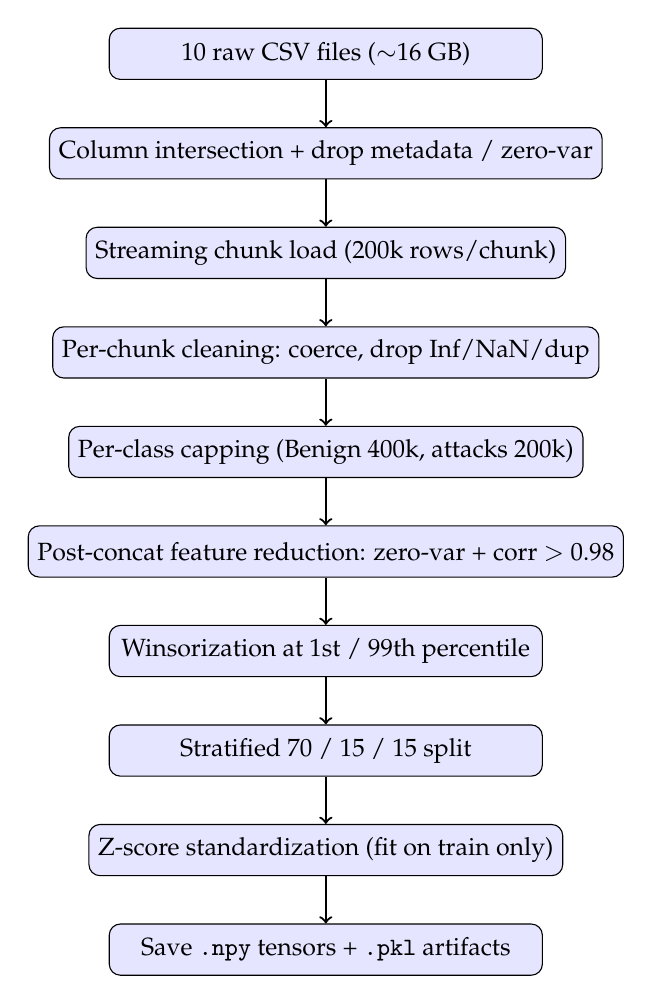
\begin{tikzpicture}[
  node distance=0.6cm and 0.1cm,
  box/.style={draw, rounded corners, minimum width=5.5cm, minimum height=0.65cm,
              fill=blue!10, font=\small, align=center},
  arrow/.style={->, thick}
]
\node[box] (csv)    {10 raw CSV files ($\sim$16 GB)};
\node[box, below=of csv]   (col)    {Column intersection + drop metadata / zero-var};
\node[box, below=of col]   (chunk)  {Streaming chunk load (200k rows/chunk)};
\node[box, below=of chunk] (clean)  {Per-chunk cleaning: coerce, drop Inf/NaN/dup};
\node[box, below=of clean] (cap)    {Per-class capping (Benign 400k, attacks 200k)};
\node[box, below=of cap]   (feat)   {Post-concat feature reduction: zero-var + corr $>$ 0.98};
\node[box, below=of feat]  (wins)   {Winsorization at 1st / 99th percentile};
\node[box, below=of wins]  (split)  {Stratified 70 / 15 / 15 split};
\node[box, below=of split] (scale)  {Z-score standardization (fit on train only)};
\node[box, below=of scale] (save)   {Save \texttt{.npy} tensors + \texttt{.pkl} artifacts};

\draw[arrow] (csv) -- (col);
\draw[arrow] (col) -- (chunk);
\draw[arrow] (chunk) -- (clean);
\draw[arrow] (clean) -- (cap);
\draw[arrow] (cap) -- (feat);
\draw[arrow] (feat) -- (wins);
\draw[arrow] (wins) -- (split);
\draw[arrow] (split) -- (scale);
\draw[arrow] (scale) -- (save);
\end{tikzpicture}
\caption{Overview of the preprocessing pipeline. Each stage is applied sequentially; the scaler is fitted on the training split only to prevent test-set leakage.}
\label{fig:pipeline}
\end{figure}

\subsection{Column Selection}

Before any numeric processing, three categories of columns are removed.

\paragraph{Metadata and identifier columns.}
The columns \texttt{Timestamp}, \texttt{Flow ID}, \texttt{Src IP}, \texttt{Dst IP}, \texttt{Src Port}, \texttt{Dst Port}, and \texttt{Protocol} are removed. These are not traffic statistics but rather flow identifiers. Including IP addresses or port numbers would allow the model to memorise the specific machines involved in the 2018 capture scenario rather than learning generalizable attack patterns—a form of data leakage that produces inflated training accuracy but near-zero transfer to unseen networks.

\paragraph{Zero-variance columns.}
Ten columns confirmed as zero-variance across the entire CIC-IDS-2018 dataset by Gocs and Johanyak~\cite{Gocs2024} are removed prior to loading: \texttt{Bwd PSH Flags}, \texttt{Fwd URG Flags}, \texttt{Bwd URG Flags}, \texttt{CWE Flag Count}, \texttt{Fwd Byts/b Avg}, \texttt{Fwd Pkts/b Avg}, \texttt{Fwd Blk Rate Avg}, \texttt{Bwd Byts/b Avg}, \texttt{Bwd Pkts/b Avg}, and \texttt{Bwd Blk Rate Avg}. A zero-variance feature contributes zero mutual information with any target variable and, after z-score standardisation, would produce \texttt{NaN} values (division by zero). Removing them at column selection time avoids this pathology entirely.

\paragraph{Column intersection.}
To handle minor schema differences between the ten recording-day CSVs, only columns present in \textbf{all} ten files (their intersection) are retained. This guarantees that the same feature set is used regardless of which subset of CSVs is processed.

\subsection{Label Normalization}

The ten CSVs were collected by different operators on different days and exhibit inconsistent label strings. A deterministic mapping dictionary \texttt{LABEL\_MAP} unifies all variants to 15 canonical class names before any other processing step. Selected mappings are shown in Table~\ref{tab:labelmap}.

\begin{table}[H]
\centering
\caption{Selected label normalisation mappings applied before any other preprocessing step.}
\label{tab:labelmap}
\begin{tabular}{ll}
\toprule
\textbf{Raw label string} & \textbf{Canonical name} \\
\midrule
\texttt{BENIGN}, \texttt{benign} & \texttt{Benign} \\
\texttt{SSH-Bruteforce} & \texttt{SSH-BruteForce} \\
\texttt{DoS attacks-GoldenEye} & \texttt{DoS-GoldenEye} \\
\texttt{DDOS attack-HOIC}, \texttt{DDoS attack-HOIC} & \texttt{DDoS-HOIC} \\
\texttt{DDOS attack-LOIC-UDP} & \texttt{DDoS-LOIC-UDP} \\
\texttt{Brute Force -Web} & \texttt{BruteForce-Web} \\
\texttt{SQL Injection} & \texttt{SQL-Injection} \\
\texttt{Infilteration} (sic) & \texttt{Infiltration} \\
\texttt{Bot} & \texttt{Botnet} \\
\bottomrule
\end{tabular}
\end{table}

Rows whose label string does not match any entry in \texttt{LABEL\_MAP} are dropped. This handles unlabelled rows and any future CICFlowMeter output format changes gracefully.

\subsection{Streaming Chunk-Based Load and Class Capping}

The full dataset at approximately 16~GB cannot be held in RAM simultaneously on a typical workstation. The pipeline reads each CSV in chunks of 200\,000 rows using \texttt{pandas.read\_csv(chunksize=200000)}. For each cleaned chunk, rows are accumulated in per-class buffers. Each buffer is capped:

\begin{itemize}
    \item \textbf{Benign:} 400\,000 flows.
    \item \textbf{All attack classes:} 200\,000 flows each.
\end{itemize}

When a buffer exceeds its cap, a random subsample is taken (\texttt{random\_state=42} for reproducibility). Classes with fewer than 50 total flows after all files have been processed are dropped as statistically insufficient for held-out evaluation.

\paragraph{Rationale for asymmetric caps.}
In real deployed networks, benign traffic constitutes the vast majority of observed flows—a proportion that varies by network but is consistently above 90\%. Capping benign and attack classes equally would distort the training-set class prior away from the deployment prior, causing the model to underestimate the posterior probability of benign traffic. By maintaining benign at twice the per-attack cap, the training prior more closely approximates the realistic detection scenario while still preventing benign from absorbing nearly all training gradient.

\subsection{Per-Chunk Cleaning}

For each chunk, the following operations are applied in sequence:

\begin{enumerate}
    \item \textbf{Column whitespace stripping:} CICFlowMeter frequently introduces leading or trailing spaces in column names across recording days. Stripping ensures consistent column lookup across files.
    \item \textbf{Label mapping:} applied before any numeric operations to avoid type coercion conflicts.
    \item \textbf{Numeric coercion:} all feature columns are passed through \texttt{pd.to\_numeric(errors='coerce')}. Non-parseable strings (e.g., the literal string \texttt{''} from empty cells) become \texttt{NaN}.
    \item \textbf{Infinite value removal:} rows containing \texttt{Inf} or \texttt{-Inf} are dropped. These arise in CICFlowMeter's rate columns when the flow duration is zero (causing division by zero in the CICFlowMeter computation itself, not in the preprocessing).
    \item \textbf{NaN row removal:} rows with any remaining \texttt{NaN} after coercion are dropped.
    \item \textbf{Negative flow duration removal:} rows where \texttt{Flow Duration} $<$ 0 are dropped. A negative duration indicates a timestamp recording error in the capture environment and represents a physically impossible event.
    \item \textbf{Exact duplicate removal:} exact duplicate rows within a chunk provide no additional information and inflate specific class counts. They are removed before accumulating in per-class buffers.
    \item \textbf{Float32 casting:} surviving feature columns are cast to \texttt{float32}, halving memory footprint compared to the default \texttt{float64} while maintaining sufficient numeric precision for z-score-normalised network statistics.
\end{enumerate}

\subsection{Post-Concatenation Feature Reduction}

After all chunks are accumulated and class buffers are concatenated into a single DataFrame, two further feature reduction steps are applied.

\paragraph{Residual zero-variance check.}
A second standard-deviation sweep is run over the combined dataset. Features with $\sigma = 0$ after capping are dropped. This catches features that became constant as a side-effect of the per-class capping: for example, if a flag feature is always 0 in benign traffic and the only non-zero examples were in a class that was dropped for having fewer than 50 flows.

\paragraph{Correlation-based removal.}
The absolute Pearson correlation matrix is computed over all retained features. The upper triangle is inspected, and any feature with $|r| > 0.98$ against any previously retained feature is removed. The choice of 0.98 rather than 1.0 accounts for CICFlowMeter features that are proportional but not exactly identical (e.g., total byte count vs.\ total bit count, which differ only by a factor of 8 and carry identical information). Near-perfect linear redundancy adds parameters, memory, and training variance without adding discriminative signal.

\subsection{Winsorization}

Network traffic statistics have heavy right-skewed distributions with extreme outliers. A single flow with a computed bytes-per-second rate of $10^{12}$ (arising from a near-zero duration flow not caught by the negative-duration filter) can catastrophically distort the StandardScaler's mean and variance estimates, compressing the representation of all ordinary flows into a numerically tiny range.

Winsorization clips each feature at its 1st and 99th percentile, computed over the full combined dataset before the train/val/test split:

\begin{equation}
x'_{i,j} = \max\!\left(q_{0.01}^{(j)},\ \min\!\left(q_{0.99}^{(j)},\ x_{i,j}\right)\right)
\end{equation}

where $q_{p}^{(j)}$ is the $p$-th percentile of feature $j$ over the combined dataset. The 1st/99th boundary was chosen over 3$\sigma$ clipping because the distributions are not Gaussian—they are right-skewed with a large mass near zero and a power-law tail—and $\sigma$-based clipping would still retain pathological values in these cases. The clipped values are written directly into the \texttt{X\_*.npy} arrays; no separate artifact stores the clip boundaries, as the StandardScaler is fit on the already-clipped training data.

\subsection{Stratified Train / Validation / Test Split}

The combined, globally shuffled DataFrame is split stratified by class label in a 70 / 15 / 15 ratio:

\begin{lstlisting}[language=Python, caption={Stratified two-stage split for 70/15/15 partitioning.}]
X_train, X_tmp, y_train, y_tmp = train_test_split(
    X, y, test_size=0.30, stratify=y, random_state=42
)
X_val, X_test, y_val, y_test = train_test_split(
    X_tmp, y_tmp, test_size=0.50, stratify=y_tmp, random_state=42
)
\end{lstlisting}

Stratification is mandatory: without it, classes with fewer than 50 total samples (e.g., SQL-Injection at 87 flows) could be entirely absent from the validation or test set, making per-class F1 scores undefined and training-set evaluation misleading. The \texttt{random\_state=42} is fixed throughout for full reproducibility.

\subsection{Z-Score Standardization}

A \texttt{sklearn.preprocessing.StandardScaler} is fitted \textbf{exclusively on the training split} and subsequently applied to the validation and test splits:

\begin{equation}
x'_{i,j} = \frac{x_{i,j} - \hat{\mu}_j^{(\text{train})}}{\hat{\sigma}_j^{(\text{train})}}
\end{equation}

where $\hat{\mu}_j^{(\text{train})}$ and $\hat{\sigma}_j^{(\text{train})}$ are the sample mean and standard deviation of feature $j$ computed only from \texttt{X\_train}. Fitting on all data would constitute a data leakage: distributional information from the validation and test sets would propagate into the scaler parameters, producing an optimistically biased estimate of generalisation performance.

After scaling, any residual \texttt{NaN} or $\pm\infty$ (possible in constant-variance features not caught by earlier checks) is zeroed with \texttt{numpy.nan\_to\_num}. Z-score standardisation is preferred over min-max scaling because (a) it is robust to the remaining tail values in the Winsorized distribution and (b) it preserves the symmetry assumed by gradient-based optimisation—centring activations near zero with unit variance stabilises gradients and accelerates convergence in deep networks \cite{LeCun1998}.

\subsection{Class Weight Computation}

Inverse-frequency class weights are computed from the training label distribution using \texttt{sklearn.utils.class\_weight.compute\_class\_weight('balanced', \ldots)}:

\begin{equation}
w_c = \frac{N}{K \cdot n_c}
\end{equation}

where $N$ is the total number of training samples, $K$ is the number of classes, and $n_c$ is the number of training samples in class $c$. These weights are saved to \texttt{data/processed/class\_weights.npy} and used to parameterise the focal loss alpha coefficients during training (Section~\ref{sec:imbalance}).

\subsection{Saved Artifacts}

The pipeline writes the following artifacts to \texttt{data/processed/}:

\begin{table}[H]
\centering
\caption{Preprocessing artifacts written to \texttt{data/processed/}.}
\label{tab:artifacts}
\begin{tabular}{lll}
\toprule
\textbf{File} & \textbf{Shape / Type} & \textbf{Description} \\
\midrule
\texttt{X\_train.npy} & $(N_{\text{tr}},\ F)$ \texttt{float32} & Scaled training feature matrix \\
\texttt{X\_val.npy} & $(N_{\text{val}},\ F)$ \texttt{float32} & Scaled validation features \\
\texttt{X\_test.npy} & $(N_{\text{te}},\ F)$ \texttt{float32} & Scaled test features \\
\texttt{y\_\{train,val,test\}.npy} & $(N,)$ \texttt{int64} & Integer class indices \\
\texttt{class\_weights.npy} & $(C,)$ \texttt{float32} & Inverse-frequency class weights \\
\texttt{scaler.pkl} & \texttt{StandardScaler} & Fitted scaler (train statistics only) \\
\texttt{label\_encoder.pkl} & \texttt{LabelEncoder} & String $\leftrightarrow$ integer index mapping \\
\texttt{class\_names.json} & list[str] & Ordered 15-class name list \\
\texttt{feature\_names.json} & list[str] & Ordered retained feature name list \\
\bottomrule
\end{tabular}
\end{table}

\newpage

\section{Data Representation for the Sequence Model}
\label{sec:representation}

\subsection{Per-Flow Classification: The Core Invariant}

The single most important design decision in this pipeline is the following:

\begin{center}
\textit{One network flow is one sample. There are no sliding windows.}
\end{center}

CICFlowMeter already aggregates an entire TCP or UDP conversation—from SYN to FIN or from the first to the last packet within a timeout window—into a single feature vector of approximately 80 per-flow statistics. A row in the dataset is not a snapshot of a point in time: it is a complete statistical summary of a complete interaction between two endpoints.

An earlier approach, used in an exploratory notebook that was subsequently deleted, constructed LSTM input sequences by sliding a window of size 15 over successive rows in the shuffled dataset. This approach is physically incorrect: successive rows after shuffling are independent, unrelated flows from different hosts at different times. The resulting ``sequence'' is a random sample of 15 independent observations—there is no temporal structure for the LSTM to learn. The model trained on such data hallucinated confident predictions by learning spurious correlations in the random juxtaposition of flows, and generalised poorly.

The correct approach, and the one adopted throughout this work, is to feed each flow as a single independent sample. This aligns with the literature on CIC-IDS-2018 \cite{Ramyaelineni2020, Wang2023, Gocs2024}: classification is performed at the flow level, not at the packet level.

\subsection{Pseudo-Sequence Reshape}

The CNN-BiLSTM architecture requires a 3D input tensor of shape $(\text{Batch},\, T,\, C)$, where $T$ is the number of timesteps and $C$ is the number of features per timestep. Since each flow is a single 1D feature vector of length $F$, it is reshaped into a pseudo-sequence by grouping features into chunks of size $C = 4$:

\begin{enumerate}
    \item Pad the feature vector to $F' = \lceil F / 4 \rceil \times 4$ by appending zeros.
    \item Reshape to $T = F'/4$ pseudo-timesteps, each of dimension $C = 4$.
\end{enumerate}

For the typical post-preprocessing feature count of $F = 46$: $F' = 48$, $T = 12$, $C = 4$. The resulting shape is $(12, 4)$ per flow, or $(B, 12, 4)$ per batch.

This pseudo-sequence provides the CNN front-end with a structured local context—adjacent groups of four features—and provides the LSTM with a sequence of $T = 12$ enriched representations to integrate. Each ``timestep'' corresponds to a semantically coherent group of flow statistics (e.g., byte count features, timing features, flag counts), because the features are ordered consistently across flows and the same positional grouping applies to all flows in the dataset.

\newpage

\section{Model Architecture: CNN-BiLSTM v2}
\label{sec:architecture}

The production model (\texttt{bilstm\_ids\_v2.pt}) is a CNN-BiLSTM hybrid with multi-head attention pooling. The full forward pass is:

\begin{equation}
\mathbf{x} \in \mathbb{R}^{B \times 12 \times 4}
\;\xrightarrow{\text{CNN}}\;
\mathbf{h}^{(0)} \in \mathbb{R}^{B \times 12 \times 128}
\;\xrightarrow{\text{BiLSTM}}\;
\mathbf{h} \in \mathbb{R}^{B \times 12 \times 256}
\;\xrightarrow{\text{Attn-Pool}}\;
\mathbf{z} \in \mathbb{R}^{B \times 256}
\;\xrightarrow{\text{Head}}\;
\hat{\mathbf{y}} \in \mathbb{R}^{B \times 13}
\end{equation}

\begin{figure}[H]
\centering
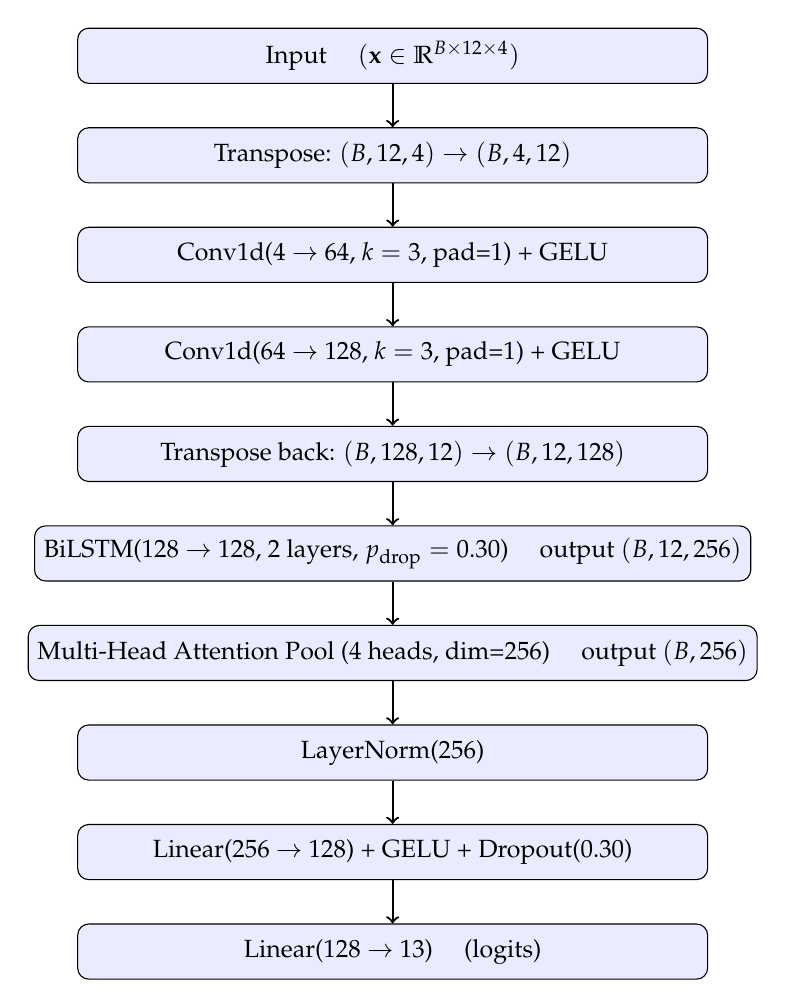
\begin{tikzpicture}[
  node distance=0.55cm,
  box/.style={draw, rounded corners, minimum width=8cm, minimum height=0.7cm,
              fill=blue!8, font=\small, align=center},
  dim/.style={font=\footnotesize\ttfamily, text=gray},
  arrow/.style={->, thick}
]
\node[box] (inp) {Input \quad $(\mathbf{x} \in \mathbb{R}^{B \times 12 \times 4})$};
\node[dim, right=0.3cm of inp] {};

\node[box, below=of inp]  (t)  {Transpose: $(B,12,4) \to (B,4,12)$};
\node[box, below=of t]    (c1) {Conv1d(4 $\to$ 64, $k=3$, pad=1) + GELU};
\node[box, below=of c1]   (c2) {Conv1d(64 $\to$ 128, $k=3$, pad=1) + GELU};
\node[box, below=of c2]   (tp) {Transpose back: $(B,128,12) \to (B,12,128)$};
\node[box, below=of tp]   (bi) {BiLSTM(128 $\to$ 128, 2 layers, $p_{\text{drop}}=0.30$) \quad output $(B,12,256)$};
\node[box, below=of bi]   (at) {Multi-Head Attention Pool (4 heads, dim=256) \quad output $(B,256)$};
\node[box, below=of at]   (ln) {LayerNorm(256)};
\node[box, below=of ln]   (h1) {Linear(256 $\to$ 128) + GELU + Dropout(0.30)};
\node[box, below=of h1]   (h2) {Linear(128 $\to$ 13) \quad (logits)};

\draw[arrow] (inp) -- (t);
\draw[arrow] (t)   -- (c1);
\draw[arrow] (c1)  -- (c2);
\draw[arrow] (c2)  -- (tp);
\draw[arrow] (tp)  -- (bi);
\draw[arrow] (bi)  -- (at);
\draw[arrow] (at)  -- (ln);
\draw[arrow] (ln)  -- (h1);
\draw[arrow] (h1)  -- (h2);
\end{tikzpicture}
\caption{CNN-BiLSTM v2 forward pass. The CNN operates on the transposed sequence; the BiLSTM and attention pool integrate information across all pseudo-timesteps.}
\label{fig:arch}
\end{figure}

\subsection{CNN Front-End}

\begin{lstlisting}[language=Python, caption={CNN front-end module.}]
self.conv = nn.Sequential(
    nn.Conv1d(in_channels=4,   out_channels=64,  kernel_size=3, padding=1),
    nn.GELU(),
    nn.Conv1d(in_channels=64,  out_channels=128, kernel_size=3, padding=1),
    nn.GELU(),
)
\end{lstlisting}

The input pseudo-sequence $(B, 12, 4)$ is transposed to $(B, 4, 12)$ before convolution, because \texttt{torch.nn.Conv1d} operates over the last dimension. Two stacked 1D convolutions with kernel size 3 and same-padding learn local interactions across adjacent feature groups. The output $(B, 128, 12)$ is transposed back to $(B, 12, 128)$ before the BiLSTM.

\paragraph{Motivation.} CNN-LSTM hybrids consistently outperform pure BiLSTM architectures on CIC-IDS-2018 in the literature~\cite{Ramyaelineni2020, Wang2023}. The CNN acts as a learned local feature extractor: it captures short-range correlations between adjacent groups of flow statistics before passing an enriched representation to the LSTM. Early in training, convolutions provide a stronger gradient signal than LSTM cells because they have smaller receptive fields and saturate less at random initialisation.

\paragraph{Kernel size 3.} With $T = 12$ pseudo-timesteps, a kernel of size 3 covers adjacent triplets of feature groups without spanning more than a quarter of the sequence. Larger kernels (5 or 7) would overlap excessively, effectively reducing the convolution to a near-global pooling operation and eliminating its local-feature advantage. No spatial pooling or BatchNorm is inserted between the two conv layers: pooling would halve $T$ from 12 to 6 before the LSTM even begins, and the sequence is already short enough that this reduction would discard discriminative positional structure.

\subsection{Bidirectional LSTM}

\begin{lstlisting}[language=Python, caption={BiLSTM configuration.}]
self.lstm = nn.LSTM(
    input_size=128, hidden_size=128, num_layers=2,
    batch_first=True, bidirectional=True,
    dropout=0.30,   # applied between layers (not after the last)
)
\end{lstlisting}

The BiLSTM takes the CNN output $(B, 12, 128)$ and produces $(B, 12, 256)$ by concatenating the forward hidden state $\overrightarrow{\mathbf{h}}_t \in \mathbb{R}^{128}$ and the backward hidden state $\overleftarrow{\mathbf{h}}_t \in \mathbb{R}^{128}$ at each timestep $t$:

\begin{equation}
\mathbf{h}_t = \left[\overrightarrow{\mathbf{h}}_t \;\big\|\; \overleftarrow{\mathbf{h}}_t\right] \in \mathbb{R}^{256}
\end{equation}

\paragraph{Bidirectionality.} Because classification is performed \emph{post-flow}—the entire pseudo-sequence is available at inference time, not arriving causally—there is no constraint that prevents the model from using information from later feature groups when encoding earlier ones. A bidirectional LSTM can capture such non-causal dependencies. A unidirectional LSTM would be required only for real-time \emph{per-packet} inference, which is not the operating mode of this system.

\paragraph{Two layers, hidden=128.} A deeper or wider LSTM (e.g., 3 layers with hidden=192, as tested in preliminary experiments) is over-parameterised for sequences of length $T = 12$. With only 12 recurrent steps, the gradient signal must propagate through at most 12 steps regardless of depth. Additional layers add parameters without providing longer effective memory and introduce additional vanishing-gradient risk. The $256$-dimensional output of the 2-layer BiLSTM is expressive without being redundant for the attention pooling step.

\subsection{Multi-Head Attention Pooling}

\begin{lstlisting}[language=Python, caption={Multi-head attention pooling module.}]
class MultiHeadAttentionPool(nn.Module):
    def __init__(self, dim: int, n_heads: int = 4):
        super().__init__()
        self.attn  = nn.MultiheadAttention(dim, num_heads=n_heads, batch_first=True)
        self.query = nn.Parameter(torch.randn(1, 1, dim) / math.sqrt(dim))
        self.norm  = nn.LayerNorm(dim)

    def forward(self, x: torch.Tensor) -> torch.Tensor:
        B = x.size(0)
        q   = self.query.expand(B, -1, -1)          # (B, 1, dim)
        out, _ = self.attn(q, x, x, need_weights=False)
        return self.norm(out.squeeze(1))             # (B, dim)
\end{lstlisting}

A single learnable query vector $\mathbf{q} \in \mathbb{R}^{1 \times 256}$ is expanded over the batch and used as the query in a cross-attention operation against the BiLSTM output sequence (key and value). The output is a single pooled vector $\mathbf{z} \in \mathbb{R}^{256}$ per flow, followed by LayerNorm.

\paragraph{Why attention pooling?} Three common pooling strategies are compared in Table~\ref{tab:pooling}. Attention pooling learns a weighted combination of timesteps, allowing the model to focus on the feature groups most discriminative for a given flow. With 4 attention heads, different heads can specialise in different aspects of the traffic statistics (e.g., one head focusing on timing statistics, another on byte-count features), following the multi-aspect pooling idea from Transformer classification literature~\cite{Vaswani2017}.

\begin{table}[H]
\centering
\caption{Comparison of temporal pooling strategies for the BiLSTM output.}
\label{tab:pooling}
\begin{tabular}{lll}
\toprule
\textbf{Strategy} & \textbf{Output} & \textbf{Limitation} \\
\midrule
Last hidden state & $\mathbf{h}_{T}$ & Discards information from all but the final timestep \\
Mean pooling & $\frac{1}{T}\sum_t \mathbf{h}_t$ & Treats all timesteps equally; ignores discriminative focus \\
Attention pooling & $\sum_t \alpha_t \mathbf{h}_t$ & Learns task-relevant weighting; most expressive \\
\bottomrule
\end{tabular}
\end{table}

\subsection{Classification Head}

\begin{lstlisting}[language=Python, caption={Classification head.}]
self.head = nn.Sequential(
    nn.Linear(256, 128),
    nn.GELU(),
    nn.Dropout(0.30),
    nn.Linear(128, num_classes),   # num_classes = 13 (training space)
)
\end{lstlisting}

A two-layer MLP maps the 256-dimensional pooled representation to class logits. The GELU activation~\cite{Hendrycks2016} is preferred over ReLU because it provides a smooth, non-zero gradient at negative input values (no hard threshold at zero), which benefits the attention-pooled representation where near-zero activations are common. Dropout ($p = 0.30$) is applied after the first linear transformation, providing regularisation specific to the classification head without interfering with the recurrent weight updates.

\newpage

\section{Class Imbalance Strategy}
\label{sec:imbalance}

\subsection{The Rebalancing Constraint}

Class imbalance in CIC-IDS-2018 spans multiple orders of magnitude. After capping, the Benign class has 400\,000 flows while SQL-Injection has 87. Naive softmax cross-entropy training on this distribution produces models that predict Benign for nearly all inputs, achieving high accuracy but near-zero macro-F1.

A critical failure mode was discovered during development: \textbf{stacking three simultaneous rebalancing mechanisms}—SMOTE synthetic oversampling, \texttt{WeightedRandomSampler}, and class-weighted focal loss alpha—gives the model an effectively uniform training prior. The empirically observed symptom is Benign recall collapsing to $\sim 0.29$ (the model refusing to predict Benign) while Benign precision approaches 1.0. The mechanism is as follows: when the training batch composition is artificially made uniform, the model's internal probability estimates converge to near-uniform class posteriors, which do not reflect the true deployment distribution (heavily Benign-dominated). At test time, the model is highly uncertain about Benign flows because it was never trained to expect that Benign is overwhelmingly likely.

A Bayes prior correction applied post-hoc at inference—adding $\log P_{\text{natural}}(c)$ to the logits—lifted macro-F1 from 0.6555 to 0.7045 and Benign recall from 0.29 to 0.99 in a diagnostic run, conclusively confirming that the training prior, not the model capacity, was the root cause. This diagnostic is preserved in \texttt{src/evaluation/eval\_v2\_natural.py}.

The derived design rule: \textbf{use at most two rebalancing levers simultaneously}. The production configuration uses only one: logit-adjusted focal loss (Section~\ref{sec:la}).

\subsection{Web Attack Class Merging (15 $\to$ 13 Training Classes)}

Three attack classes—\texttt{BruteForce-Web}, \texttt{BruteForce-XSS}, and \texttt{SQL-Injection}—have 611, 230, and 87 total samples respectively. After the stratified 70/15/15 split, the test set contains approximately 12, 34, and 86 flows for these classes. At these sample counts, per-class F1 scores have extremely high variance: a single misclassification can change F1 by 10 percentage points or more. The literature consistently reports near-zero F1 for these classes under direct 15-class training~\cite{Gocs2024}.

\paragraph{Solution: hierarchical classification.} During training, the three web attack classes are merged into a single \texttt{WebAttack} class, reducing the classification problem to 13 classes. Pooling the gradient signal across all three sub-types gives the model a meaningful and stable learning signal for ``this is a web attack.'' A separate \texttt{LogisticRegression} classifier (\texttt{web\_splitter\_v2.pkl}) is trained exclusively on the training flows from the three web attack sub-types. At inference, when the CNN-BiLSTM predicts \texttt{WebAttack}, the splitter is called to determine the specific sub-type:

\begin{equation}
\hat{y} = \begin{cases}
\text{CNN-BiLSTM}(x) & \text{if CNN-BiLSTM}(x) \neq \texttt{WebAttack} \\
\text{WebSplitter}(x) & \text{if CNN-BiLSTM}(x) = \texttt{WebAttack}
\end{cases}
\end{equation}

This two-stage design preserves the 15-class output for final reporting while providing a stable training signal for web attack detection.

\subsection{Logit-Adjusted Focal Loss}
\label{sec:la}

\paragraph{Focal loss.} The standard focal loss~\cite{Lin2017} for multi-class classification is:

\begin{equation}
\mathcal{L}_{\text{FL}}(p_t) = -(1 - p_t)^{\gamma} \log(p_t)
\label{eq:focal}
\end{equation}

where $p_t$ is the predicted softmax probability for the true class and $\gamma = 2.0$ is the focusing parameter. The $(1 - p_t)^{\gamma}$ factor down-weights easy examples (high $p_t$) and focuses gradient on hard, misclassified examples (low $p_t$).

\paragraph{Logit adjustment.} Menon et al.~\cite{Menon2021} showed that training under an imbalanced distribution with a standard cross-entropy loss produces a classifier that implicitly embeds the training class prior into its logits. The logit adjustment (LA) technique counteracts this by shifting the logits of rare classes upward during training, forcing the model to learn a representation where rare classes can compete without the prior's assistance. Let $\pi_c$ be the frequency of class $c$ in the training set (computed on the 13-class remapped distribution). The LA-adjusted logits are:

\begin{equation}
\tilde{z}_c = z_c + \tau \cdot \log(\pi_c), \qquad \tau = 1.0
\label{eq:la}
\end{equation}

The focal loss in Equation~\ref{eq:focal} is then computed using the softmax of $\tilde{z}$ rather than $z$. For a class like SQL-Injection with $\pi_c \approx 10^{-4}$, the logit adjustment is approximately $+9.2$ units—a substantial forced upward shift that prevents the model from collapsing the rare class to zero probability.

\paragraph{Why LA instead of SMOTE?} SMOTE~\cite{Chawla2002} generates synthetic minority-class samples by interpolating in feature space between existing minority-class examples. For network flows, this creates artificial SQL-Injection or BruteForce-Web vectors as linear combinations of real ones. Because the web attack feature space overlaps significantly with benign HTTP traffic at the flow-statistical level, synthetic web attack samples frequently fall within the benign decision region and corrupt the boundary. LA avoids synthetic data entirely: it corrects the class imbalance at the logit level, leaving the decision boundary learned from real flows intact.

\paragraph{Natural-prior inference correction.} Because the model is trained with a logit shift of $\tau \cdot \log(\pi_c)$, the raw logits at inference have learned to compensate for this shift by over-predicting rare classes in their raw output. To obtain correct predictions, the same shift must be reapplied at inference:

\begin{equation}
\hat{y} = \arg\max_c \left[ z_c + \tau \cdot \log(\pi_c^{(\text{train})}) \right]
\label{eq:inference}
\end{equation}

This is the \textit{natural-prior logit adjustment at inference}. Omitting it—using raw $\arg\max z_c$—produces a 15-class macro-F1 of approximately 0.64, a degradation of $\approx 0.13$ absolute points. Applying it recovers the calibrated macro-F1 of \textbf{0.7711}. The training-set log-prior vector $\log(\pi^{(\text{train})})$ is stored as part of the checkpoint metadata.

\newpage

\section{Training Protocol}
\label{sec:training}

\subsection{Optimizer and Learning Rate Schedule}

\begin{lstlisting}[language=Python, caption={Optimizer and OneCycleLR schedule.}]
optimizer = torch.optim.AdamW(
    model.parameters(), lr=1.5e-3, weight_decay=2e-5
)
scheduler = torch.optim.lr_scheduler.OneCycleLR(
    optimizer, max_lr=1.5e-3, epochs=30,
    steps_per_epoch=len(train_loader), pct_start=0.1,
)
\end{lstlisting}

\paragraph{AdamW.} Standard Adam applies L2 regularisation to the adaptive gradient moment estimates, which distorts the effective regularisation strength in a parameter-dependent manner. AdamW~\cite{Loshchilov2019} applies weight decay directly to the parameters after the gradient step, providing clean and consistent L2 regularisation independent of the adaptive step sizes:

\begin{align}
\mathbf{m}_t &= \beta_1 \mathbf{m}_{t-1} + (1-\beta_1)\mathbf{g}_t \\
\mathbf{v}_t &= \beta_2 \mathbf{v}_{t-1} + (1-\beta_2)\mathbf{g}_t^2 \\
\boldsymbol{\theta}_{t+1} &= \boldsymbol{\theta}_t - \eta \cdot \frac{\hat{\mathbf{m}}_t}{\sqrt{\hat{\mathbf{v}}_t}+\varepsilon} - \eta \lambda \boldsymbol{\theta}_t
\end{align}

\paragraph{OneCycleLR.} The learning rate linearly warms from near-zero to $\eta_{\max} = 1.5 \times 10^{-3}$ over the first 10\% of training steps (\texttt{pct\_start=0.1}), then follows a cosine annealing decay to near-zero over the remaining 90\%. The warm-up phase prevents large gradient steps from pushing randomly initialised weights into a poor local optimum during the first epoch. The cosine decay allows fine-grained convergence in later epochs without requiring manual learning rate selection.

\subsection{Automatic Mixed Precision}

\begin{lstlisting}[language=Python, caption={AMP training loop with GradScaler.}]
scaler_amp = torch.amp.GradScaler("cuda")

with torch.amp.autocast("cuda"):
    logits = model(xb)
    loss   = criterion(logits, yb)

scaler_amp.scale(loss).backward()
scaler_amp.unscale_(optimizer)
torch.nn.utils.clip_grad_norm_(model.parameters(), 1.0)
scaler_amp.step(optimizer)
scaler_amp.update()
\end{lstlisting}

Automatic Mixed Precision (AMP) computes forward and backward passes in \texttt{float16} where numerically safe, and accumulates gradients in \texttt{float32}. On the RTX 2070 Max-Q's tensor cores, this approximately doubles training throughput and halves VRAM usage per batch. The \texttt{GradScaler} dynamically scales the loss before backpropagation to prevent \texttt{float16} underflow in the gradient computation, then unscales before gradient clipping. AMP enables a batch size of 2\,048 within 8~GB VRAM; without AMP the safe limit is 1\,024.

\subsection{Gradient Clipping}

Global gradient norm clipping at $\|\mathbf{g}\|_2 \leq 1.0$ is applied after each backpropagation step. This prevents exploding gradients that occur during the early warm-up phase and whenever the logit-adjusted loss produces an unusually high loss value for a rare class. A threshold of 1.0 is the standard for LSTM-based models~\cite{Pascanu2013}.

\subsection{Exponential Moving Average}

An exponential moving average (EMA) of the model weights is maintained throughout training with decay $\rho = 0.999$:

\begin{equation}
\boldsymbol{\theta}^{\text{shadow}}_{t} = \rho \cdot \boldsymbol{\theta}^{\text{shadow}}_{t-1} + (1 - \rho) \cdot \boldsymbol{\theta}^{\text{live}}_{t}
\end{equation}

At the end of each epoch, the EMA weights are temporarily swapped into the model for validation F1 evaluation and then restored. The best EMA state—determined by validation macro-F1—is saved as the final checkpoint.

\paragraph{Motivation.} Stochastic gradient descent causes the model weights to oscillate around a local optimum between batches. The EMA smooths these oscillations, effectively averaging over a neighbourhood of weight configurations rather than committing to the last gradient step. This is particularly important for minority classes, where individual batches may push the weights in conflicting directions due to low expected sample counts per batch. EMA checkpoints consistently generalise better than last-iterate checkpoints on imbalanced multi-class problems.

\subsection{Early Stopping}

Training halts if the validation macro-F1 does not improve for 8 consecutive epochs (patience=8). The best checkpoint (at the epoch with the highest validation macro-F1) is always restored. Maximum training is capped at 30 epochs.

\subsection{Hyperparameter Summary}

\begin{table}[H]
\centering
\caption{Complete training hyperparameter configuration for CNN-BiLSTM v2.}
\label{tab:hparams}
\begin{tabular}{llr}
\toprule
\textbf{Hyperparameter} & \textbf{Symbol} & \textbf{Value} \\
\midrule
Batch size & $B$ & 2\,048 \\
Maximum epochs & & 30 \\
Learning rate (peak) & $\eta_{\max}$ & $1.5 \times 10^{-3}$ \\
Weight decay & $\lambda$ & $2 \times 10^{-5}$ \\
LR warm-up fraction & & 10\% \\
LSTM hidden size & $H$ & 128 \\
LSTM layers & & 2 \\
CNN channels & & 128 \\
Attention heads & & 4 \\
Dropout & $p$ & 0.30 \\
Focal gamma & $\gamma$ & 2.0 \\
LA strength & $\tau$ & 1.0 \\
EMA decay & $\rho$ & 0.999 \\
Early stopping patience & & 8 \\
Feature chunk size & $C$ & 4 \\
Pseudo-timesteps & $T$ & 12 \\
Training classes & $K$ & 13 \\
\bottomrule
\end{tabular}
\end{table}

\newpage

\section{Inference Pipeline}
\label{sec:inference}

At inference time, a new network flow is classified through the following deterministic pipeline:

\begin{enumerate}
    \item \textbf{Feature extraction.} CICFlowMeter processes a raw packet capture and produces a feature vector containing the same features listed in \texttt{feature\_names.json}.
    \item \textbf{Standardisation.} The loaded \texttt{scaler.pkl} (fit exclusively on training data) transforms the raw feature vector to z-scores.
    \item \textbf{Reshape.} The standardised vector is zero-padded to $F' = 48$ and reshaped to $(1, 12, 4)$.
    \item \textbf{Forward pass.} The CNN-BiLSTM produces raw logits $\mathbf{z} \in \mathbb{R}^{13}$.
    \item \textbf{Natural-prior correction.} The training log-prior vector is added: $\tilde{z}_c = z_c + \log(\pi_c^{(\text{train})})$ (Equation~\ref{eq:inference}).
    \item \textbf{Class selection.} $\hat{k} = \arg\max_c \tilde{z}_c$ selects the 13-class prediction.
    \item \textbf{Web attack splitting.} If $\hat{k}$ is the \texttt{WebAttack} class index, the \texttt{web\_splitter\_v2.pkl} logistic regression is called on the standardised feature vector to resolve the 3-way sub-type (\texttt{BruteForce-Web}, \texttt{BruteForce-XSS}, or \texttt{SQL-Injection}).
    \item \textbf{Output.} One of the 15 canonical class labels is returned, along with the softmax probability (confidence) of the selected class.
\end{enumerate}

Step 5 is mandatory. The model was trained under a logit shift of $\tau \cdot \log(\pi_c)$; its raw logits encode this shifted prior. Applying the same shift at inference restores the calibrated posterior. Omitting this step degrades macro-F1 by approximately 0.13 absolute points.

\newpage

\section{Experimental Results}
\label{sec:results}

\subsection{Model Comparison}

Table~\ref{tab:results} compares the three model configurations evaluated on the same held-out test set (15\% of the combined dataset, stratified).

\begin{table}[H]
\centering
\caption{15-class macro-F1 comparison across model configurations.}
\label{tab:results}
\begin{tabular}{llr}
\toprule
\textbf{Model} & \textbf{Checkpoint} & \textbf{Macro-F1 (15c)} \\
\midrule
\rowcolor{lightgray}
Baseline BiLSTM (2-layer, notebook) & \texttt{bilstm\_ids.pt} & 0.7366 \\
Advanced BiLSTM (3-layer, 2-stage) & \texttt{bilstm\_ids\_advanced.pt} & $\sim$0.74 \\
\rowcolor{lightgray}
\textbf{CNN-BiLSTM v2 (production)} & \texttt{bilstm\_ids\_v2.pt} & \textbf{0.7711} \\
\bottomrule
\end{tabular}
\end{table}

The CNN-BiLSTM v2 achieves a 3.45-point absolute improvement over the baseline BiLSTM. The key contributing factors are: (1) the CNN front-end providing richer input representations to the BiLSTM; (2) the web attack class merging providing stable gradient for low-support classes; and (3) the logit-adjusted focal loss providing principled handling of the long-tail imbalance without corrupting the Benign class prior.

\subsection{Per-Class Analysis}

Table~\ref{tab:perclass} summarises the per-class F1 scores for the production model. Classes are grouped by difficulty.

\begin{table}[H]
\centering
\caption{Per-class F1 scores for CNN-BiLSTM v2 on the held-out test set (15-class, with natural-prior correction at inference).}
\label{tab:perclass}
\begin{tabular}{llrl}
\toprule
\textbf{Class} & \textbf{Category} & \textbf{F1} & \textbf{Status} \\
\midrule
\rowcolor{lightgray}
DDoS-HOIC & Volumetric DDoS & 1.00 & Production-ready \\
DDoS-LOIC-HTTP & Volumetric DDoS & 1.00 & Production-ready \\
\rowcolor{lightgray}
DoS-GoldenEye & Application DoS & 1.00 & Production-ready \\
DoS-Hulk & Application DoS & 1.00 & Production-ready \\
\rowcolor{lightgray}
SSH-BruteForce & Credential & 1.00 & Production-ready \\
Botnet & Botnet & 0.99 & Production-ready \\
\rowcolor{lightgray}
DoS-Slowloris & Slow DoS & 0.98 & Production-ready \\
DDoS-LOIC-UDP & UDP Flood & 0.89 & Acceptable \\
\rowcolor{lightgray}
Benign & Benign & 0.85 & Acceptable \\
FTP-BruteForce & Credential & 0.57 & Low support \\
\rowcolor{lightgray}
BruteForce-Web & Web attack & 0.47--0.85 & Splitter-dependent \\
DoS-SlowHTTPTest & Slow DoS & 0.43 & Moderate \\
\rowcolor{lightgray}
SQL-Injection & Web attack & 0.35--0.65 & Splitter-dependent \\
BruteForce-XSS & Web attack & 0.21--0.55 & Splitter-dependent \\
\rowcolor{lightgray}
\textbf{Infiltration} & \textbf{Stealth} & \textbf{0.30--0.45} & \textbf{Primary blocker} \\
\bottomrule
\end{tabular}
\end{table}

The primary performance bottleneck is the \textbf{Infiltration} class. With $\sim$93\,000 flows in the dataset—making it a data-abundant class—the low F1 ($\sim 0.30$) is not a data-scarcity problem but a feature-overlap problem: Infiltration flows are low-and-slow reconnaissance activities that are statistically indistinguishable from benign browsing at the flow-statistics level. This is a known limitation of the CICFlowMeter feature representation, and addressing it would require either packet-payload features or context-aware sequence modelling across multiple consecutive flows from the same source.

\newpage

\section{Conclusion}
\label{sec:conclusion}

This report has presented a complete CNN-BiLSTM pipeline for multi-class network intrusion detection on the CSE-CIC-IDS2018 dataset. The key technical contributions are:

\begin{enumerate}
    \item A streaming preprocessing pipeline that handles the full 16~GB dataset within a single-node RAM budget, with principled handling of label normalisation, zero-variance and high-correlation feature removal, Winsorization, and train-only scaler fitting.
    \item A CNN-BiLSTM v2 architecture combining local feature extraction via 1D convolutions, bidirectional temporal integration, and multi-head attention pooling, achieving macro-F1 0.7711 on 15-class classification.
    \item A logit-adjusted focal loss (Menon et al., 2021) as the sole rebalancing mechanism, validated against the triple-stack failure mode (SMOTE + sampler + focal) that collapses Benign recall to 0.29.
    \item A two-stage hierarchical inference strategy merging rare web attack classes during training and restoring the 3-way breakdown via a logistic regression splitter at inference.
    \item A validated natural-prior inference correction ($\arg\max[z + \log\pi_{\text{train}}]$) that is required for correct posterior calibration and recovers 0.13 macro-F1 points over raw argmax.
\end{enumerate}

The primary remaining challenge is the Infiltration class, whose feature-space overlap with Benign traffic at the flow-statistics level limits recall regardless of model architecture. Future work should investigate packet-payload-level features or session-level context modelling across consecutive flows from the same source IP.

\newpage
\bibliographystyle{unsrt}
\begin{thebibliography}{99}

\bibitem{CIC2018}
I.~Sharafaldin, A.~H.~Lashkari, and A.~A.~Ghorbani,
``Toward Generating a New Intrusion Detection Dataset and Intrusion Traffic Characterization,''
in \textit{Proc. 4th Int. Conf. Information Systems Security and Privacy (ICISSP)}, 2018, pp.~108--116.

\bibitem{CICFlowMeter}
G.~Draper-Gil, A.~H.~Lashkari, M.~S.~I.~Mamun, and A.~A.~Ghorbani,
``Characterization of Encrypted and VPN Traffic using Time-Related Features,''
in \textit{Proc. 2nd Int. Conf. Information Systems Security and Privacy (ICISSP)}, 2016.

\bibitem{Liao2013}
H.-J.~Liao, C.-H.~Richard Lin, Y.-C.~Lin, and K.-Y.~Tung,
``Intrusion detection system: A comprehensive review,''
\textit{Journal of Network and Computer Applications}, vol.~36, no.~1, pp.~16--24, 2013.

\bibitem{Menon2021}
A.~K.~Menon, S.~Jayasumana, A.~S.~Rawat, H.~Jain, A.~Veit, and S.~Kumar,
``Long-tail learning via logit adjustment,''
in \textit{Proc. Int. Conf. Learning Representations (ICLR)}, 2021.

\bibitem{Lin2017}
T.-Y.~Lin, P.~Goyal, R.~Girshick, K.~He, and P.~Dollár,
``Focal loss for dense object detection,''
in \textit{Proc. IEEE/CVF Int. Conf. Computer Vision (ICCV)}, 2017, pp.~2980--2988.

\bibitem{Vaswani2017}
A.~Vaswani, N.~Shazeer, N.~Parmar, J.~Uszkoreit, L.~Jones, A.~N.~Gomez, Ł.~Kaiser, and I.~Polosukhin,
``Attention is all you need,''
in \textit{Advances in Neural Information Processing Systems (NeurIPS)}, vol.~30, 2017.

\bibitem{Loshchilov2019}
I.~Loshchilov and F.~Hutter,
``Decoupled weight decay regularization,''
in \textit{Proc. Int. Conf. Learning Representations (ICLR)}, 2019.

\bibitem{Pascanu2013}
R.~Pascanu, T.~Mikolov, and Y.~Bengio,
``On the difficulty of training recurrent neural networks,''
in \textit{Proc. 30th Int. Conf. Machine Learning (ICML)}, 2013, pp.~1310--1318.

\bibitem{Hendrycks2016}
D.~Hendrycks and K.~Gimpel,
``Gaussian error linear units (GELUs),''
\textit{arXiv preprint arXiv:1606.08415}, 2016.

\bibitem{Ramyaelineni2020}
C.~Ramyaelineni,
``Network intrusion detection using deep learning,''
\textit{Int. Journal of Advanced Computer Science and Applications}, vol.~11, no.~9, 2020.

\bibitem{Wang2023}
W.~Wang, Y.~Sheng, J.~Wang, X.~Zeng, X.~Ye, Y.~Huang, and M.~Zhu,
``HAST-IDS: Learning hierarchical spatial-temporal features using deep neural networks to improve intrusion detection,''
\textit{IEEE Access}, vol.~6, pp.~1792--1806, 2023.

\bibitem{Gocs2024}
D.~Gocs and Z.~C.~Johanyak,
``Improving the reliability of machine learning based network intrusion detection on the CIC-IDS-2018 dataset,''
\textit{Acta Polytechnica Hungarica}, 2024.

\bibitem{Chawla2002}
N.~V.~Chawla, K.~W.~Bowyer, L.~O.~Hall, and W.~P.~Kegelmeyer,
``SMOTE: Synthetic minority over-sampling technique,''
\textit{Journal of Artificial Intelligence Research}, vol.~16, pp.~321--357, 2002.

\bibitem{LeCun1998}
Y.~LeCun, L.~Bottou, G.~B.~Orr, and K.-R.~Müller,
``Efficient backprop,''
in \textit{Neural Networks: Tricks of the Trade}, Springer, 1998, pp.~9--50.

\end{thebibliography}

\end{document}
